\chapter{Régression Linéaire/Polynomiale/Logistique}

\myminitoc

SOON !!!

\sect{Introduction}

On va considérer des modèles $h$ sous forme linéaire.
$$ h_\theta(x) = \sum_{i = 0}^n \theta_i x_i = \theta^\trans x $$
On posera toujours $x_0 = 1$ pour avoir une ordonnée à l'origine. Le but sera alors de trouver $\theta \in \R^{n+1}$ pour que $h$ fasse des prédictions précises.

\begin{center}
	\begin{tikzpicture}[thick, >={latex}]
		\draw[->, blue] (0, 0) -- (6, 0);
		\draw[->, blue] (0, 0) -- (0, 4);
		\draw[fill] (0.357143, 0.395123) circle (0.10);
		\draw[fill] (1.146921, 1.641947) circle (0.10);
		\draw[fill] (1.740568, 1.906676) circle (0.10);
		\draw[fill] (1.835173, 1.007108) circle (0.10);
		\draw[fill] (2.915078, 2.585541) circle (0.10);
		\draw[fill] (3.815745, 2.650688) circle (0.10);
		\draw[fill] (4.439558, 2.812134) circle (0.10);
		\draw[domain=0:5.000000, smooth, variable=\x, red] 
			plot ({\x}, {0.568668 + \x * 0.554981});
		\draw [decorate, decoration={brace,amplitude=2pt}, xshift=-0.1cm, greenTikz]
			(0, 0) -- node [left] {$\theta_0$} (0, 0.568);
		\draw[dashed] (1.835, 1) -- (1.835, 1.59);
		\draw [decorate, decoration={brace,amplitude=2pt}, xshift=0.2cm, greenTikz]
			(1.835, 1.59) -- node [right] {$h_\theta(x) - y$} (1.835, 1);
	\end{tikzpicture}
\end{center}

On se posera alors le \textbf{problème des moindres carrées} :
$$ \min_\theta J(\theta) = \min_\theta \dfrac{1}{2m} \sum_{i = 1}^m \left( h_\theta(x^{(i)}) - y^{(i)} \right)^2 $$
Il y a plusieurs méthodes pour minimiser $J(\theta)$ :
\begin{itemize}
	\item \textbf{Descente de gradient par batchs}
	\item \textbf{Descente de gradient stochastique}
	\item \textbf{Descente de gradient par mini-batchs}
	\item \textbf{Solution de forme fermée}
\end{itemize}

\sect{Régression linéaire et polynomiale}

\subs{Descente de gradient}

\subsubs{Descente de gradient par batchs}

\paragraph{Idée basique}
Si $J(\theta)$ est différentiable, l'idée est la suivante :
\begin{itemize}
	\item Initialiser $\theta$ avec la valeur 0 ou par un vecteur aléatoire.
	\item Mettre à jour $\theta$ de manière à réduire $J(\theta)$ après avoir calculer les dérivées partielles de $J(\theta)$.
	\item Puis répéter ce processus jusqu'à convergence vers un minimum de $J(\theta)$.
\end{itemize}
La formule de mise à jour de $\theta$ est la suivant :
$$ \theta_i \gets \theta_i - \alpha \dfrac{\partial}{\partial \theta_i} J(\theta) $$
Où $\alpha$ est une constante qui s'appelle le \textbf{taux d'apprentissage} et qui permet de contrôler la grandeur des pas que l'on fait. \\
En utilisant la notation du gradient : $ \nabla_\theta J = \begin{bmatrix}
\frac{\partial}{\partial \theta_0} \\ \vdots \\ \frac{\partial}{\partial \theta_n}
\end{bmatrix} $, on peut réécrire la mise à jour comme cela :
\begin{center}
	\boldmath \fbox{$ \displaystyle \theta \gets \theta - \alpha \nabla_\theta J$}
\end{center}

\paragraph{Mise à jour du $i$-ème paramètre}
On se place dans le cas où $m = 1$. C'est à dire :
$$ J(\theta) = \dfrac{1}{2} (h_\theta(x) - y)^2 $$
On calcule alors la dérivée partielle selon $\theta_i$ :
$$ \begin{array}{lll}
	\dfrac{\partial}{\partial \theta_i} J(\theta)
	& = & \dfrac{\partial}{\partial \theta_i} \dfrac{1}{2} (h_\theta(x) - y)^2 \\
	& = & 2 \times \dfrac{1}{2} (h_\theta(x) - y) \times \dfrac{\partial}{\partial \theta_i}  (h_\theta(x) - y) \\
	& = & (h_\theta(x) - y) \times \dfrac{\partial}{\partial \theta_i}  (\theta_0 x_0 + ... + \theta_i x_i + ... + \theta_n x_n - y) \\
	& = & (h_\theta(x) - y) x_i
\end{array} $$
Ce qui nous permet d'avoir : $ \theta_i \gets \theta_i - \alpha (h_\theta(x) - y) x_i $. \\
Dans le cas générale on obtient alors :
\begin{center}
	\boldmath \fbox{$ \displaystyle \theta_i \gets \theta_i - \alpha \dfrac{1}{m} \sum_{j = 1}^m \left( h_\theta(x^{(j)}) - y^{(j)} \right) x_i^{(j)}$}
\end{center}
A noter qu'on parle de batch car à chaque descente de gradient on regarde l'ensemble d'entraînement en entier.

\REM{
	Avec des initialisation légèrement différentes, on peut converger vers des minimums locaux complètement différents
	\begin{center}
		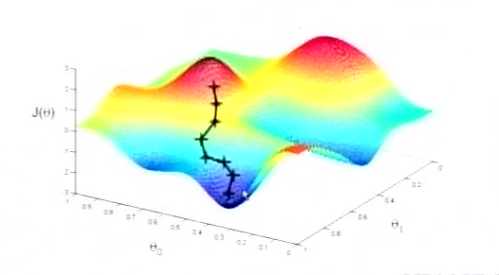
\includegraphics[scale=1.6]{grad1.png}
		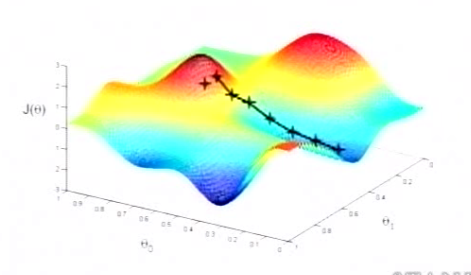
\includegraphics[scale=1.6]{grad2.png}
	\end{center}
}

\paragraph{Choix de $\alpha$}
Il est important de bien choisir $\alpha$, car si sa valeur est trop élevé il est possible que $J(\theta)$ croisse. Une valeur faible de $\alpha$ est donc préférable mais il faut savoir que plus sa valeur est faible, plus le temps de convergence sera long ...
\begin{center}
	\begin{tikzpicture}[thick, >={latex}, scale=0.9]
		\draw[domain=1.181978:6.956124, smooth, variable=\x, blue] 
			plot ({\x}, {0.5 * (\x - 4)^2});
		\draw[->, greenTikz]
			(2.000000, 2.000000) -- node[right] {\footnotesize petit $\alpha$} (3.500000, 0.125000);
		\draw[->, red]
			(2.000000, 2.000000) -- node[below] {\footnotesize grand $\alpha$} (6.160000, 2.332800);
		\draw[->, greenTikz] (3.500000, 0.125000) -- (3.875000, 0.007812);
		\draw[->, red] (6.160000, 2.332800) -- (1.667200, 2.720978);
		\draw[->, greenTikz] (3.875000, 0.007812) -- (3.968750, 0.000488);
		\draw[->, red] (1.667200, 2.720978) -- (6.519424, 3.173749);
		\draw[fill] (2, 2) circle (0.1);
	\end{tikzpicture}
\end{center}

\paragraph{Pour}
\begin{itemize}
	\item Peu de mises à jour sont nécessaires car le gradient est stable.
	\item La séparation en somme de la mise à jour permet d'utiliser des algorithmes parallèles
\end{itemize}
\paragraph{Contre}
\begin{itemize}
	\item La stabilité du gradient peu conduire prématurément vers un minimum local pas très optimal.
	\item La mise à jour peut prendre beaucoup de temps pour de grandes bases de données.
\end{itemize}

\subsubs{Descente de gradient stochastique}

Si la base de donnée est grande, disons 1 million d'exemples alors à chaque itération de le descente de gradient par batchs, on doit réaliser une somme d'erreur sur un million d'exemples. Pour plus de rapidité il nous faut donc penser à un autre algorithme où l'on fait des mises à jour de $\theta$ plus régulièrement :

\begin{center}
	\begin{algorithm}[H]
		Initialisation de $\theta$\;
		\Repeat{convergence de $J(\theta)$}{
			\For{$j=1$ à $m$}{
				$\forall i, \; \theta_i \gets \theta_i - \alpha \left( h_\theta(x^{(j)}) - y^{(j)} \right) x_i^{(j)} $
			}
		}
		\caption{Descente de gradient stochastique}
	\end{algorithm}
\end{center}

\paragraph{Pour}
\begin{itemize}
	\item La fréquence élevé des mises à jour qui peut donner un apprentissage plus rapide.
	\item Ces mise à jours un peu "chaotiques" et instables peuvent empêcher de converger vers des minimas locaux.
	\item Cet algorithme permet aussi d'avoir un acquisition de données en ligne.
\end{itemize}
\paragraph{Contre}
L'algorithme ne converge pas vers le minimum globale mais il a tendance à rester autour.

\paragraph{Descente de gradient par mini-batchs}
Pour gagner en robustesse et garder l'efficacité de la descente stochastique, on peut séparer l'ensemble d'entraînement en de petits sous-ensembles (des petits batchs). Puis on reprend la descente stochastique mais au lieu de mettre à jour $\theta$ en s'appuyant sur un seul exemple à la fois, on le met à jour en fonction de l'erreur sur un mini-batch.

\subs{Solution de forme fermée}

On pose les vecteurs et matrices suivantes :
$$ x^{(j)} = \begin{pmatrix} x_0^{(j)} \\ \vdots \\ x_n^{(j)} \end{pmatrix} \qquad
X = \begin{pmatrix} {x^{(1)}}^\trans \\ \vdots \\ {x^{(m)}}^\trans \end{pmatrix} \qquad 
\theta = \begin{pmatrix} \theta_0 \\ \vdots \\ \theta_n \end{pmatrix} \qquad
y = \begin{pmatrix} y^{(1)} \\ \vdots \\ y^{(m)} \end{pmatrix} $$
Cela nous permet de réécrire $J(\theta)$.
$$ J(\theta) = \dfrac{1}{2m} (X\theta - y)^\trans (X\theta - y) $$
En un minimum de $J$, le gradient est nul. On cherche donc à résoudre :
$$ \nabla_\theta \dfrac{1}{2} (X\theta - y)^\trans (X\theta - y) = 0 $$
\newpage

$$ \begin{array}{lll}
\nabla_\theta \dfrac{1}{2} (X\theta - y)^\trans (X\theta - y)
& = & \dfrac{1}{2} \nabla_\theta \left( \theta^\trans X^\trans X \theta - \theta^\trans X^\trans y - y^\trans X \theta + y^\trans y \right) \\ \\
& = & \dfrac{1}{2} \left[ \nabla_\theta \left(\theta^\trans X^\trans X \theta \right) - 2 \nabla_\theta \left( y^\trans X \theta \right) \right] \\ \\
& = & X^\trans X \theta - X^\trans y
\end{array} $$

\PROP[ (Solution de forme fermée)]{
	Ainsi, si $X^\trans X$ est inversible, l'expression de $\theta$ suivante est optimale :
	\vspace{-1mm}
	$$\theta = (X^\trans X)^{-1} X^\trans y$$
	En revanche si $X^\trans X$ n'est pas inversible, il est possible que des features soient redondants. Appliqué l'algorithme PCA peut alors être une solution.
}

\subs{Régression polynomiale}

Dans le cas d'une régression polynomiale, on $h_\theta(x) = \theta_0 + \theta_1 x + \theta_2 x^2 + ... + \theta_n x^n$. La fonction est toujours linéaire selon $\theta$. L'idée est alors de se placer en dimension $n+1$, en posant $x_i = x^i$.

\sect{Interprétation probabiliste de la régression}

On peut se poser la question : Pourquoi les moindres carrées ? Pourquoi ne pas minimiser la valeur absolue ou encore la puissance 4 ?

Supposons que l'erreur sur $y^{(i)}$ suit une loi gaussienne. Ceci est justifié par le théorème centrale limite. On a donc :
$$ y^{(i)} = \theta^\trans x^{(i)} + \epsilon^{(i)} $$
Où $\epsilon^{(i)} \sim \mathcal{N}(0, \sigma)$. \\
On va ensuite chercher à maximiser la vraisemblance de $y$.

\DEF{
	Soit $X_1, ..., X_m$ des variables aléatoires i.i.d de densité $f(x|\theta)$ où $\theta$ est un paramètre de la loi. Pour un échantillon $X_1 = x_1, ..., X_n = x_n$ donné, la \textbf{vraisemblance} est : \vspace{-3mm}
	$$ L(\theta) = f(x_1, ..., x_n) = \prod_{i=1}^m f(x_i|\theta) $$
	\vspace{-7mm}
}

On a donc dans notre cas :
$$ L(\theta) = \Pp(y | X, \theta) = \prod_{i=1}^m \Pp(y^{(i)} | x^{(i)}, \theta) = \prod_{i=1}^m \dfrac{1}{\sqrt{2 \pi} \sigma} \exp \left( - \dfrac{(y^{(i)} - \theta^\trans x^{(i)})^2}{2 \sigma^2} \right) $$
Une bonne manière d'étudier la vraisemblance est de la passer au logarithme car elle est souvent log-concave. La log-vraisemblance est notée $l(\theta) = \ln L(\theta)$. Voici alors ce qu'on obtient si on simplifie l'expression de la log-vraisemblance :

$$ \begin{array}{lll}
	l(\theta)
	& = & \displaystyle \sum_{i = 1}^m \ln \left( \dfrac{1}{\sqrt{2 \pi} \sigma} \exp \left( - \dfrac{(y^{(i)} - \theta^\trans x^{(i)})^2}{2 \sigma^2} \right) \right) \\
	& = & \displaystyle \sum_{i = 1}^m \ln \dfrac{1}{\sqrt{2 \pi} \sigma} + \sum_{i = 1}^m \left( \exp \left( - \dfrac{(y^{(i)} - \theta^\trans x^{(i)})^2}{2 \sigma^2} \right) \right) \\
	& = & \displaystyle m \ln \dfrac{1}{\sqrt{2 \pi} \sigma} - \sum_{i = 1}^m \dfrac{(y^{(i)} - \theta^\trans x^{(i)})^2}{2 \sigma^2}
\end{array} $$
Ainsi maximiser $l(\theta)$ revient à minimiser $\displaystyle J(\theta) = \sum_{i = 1}^m \dfrac{(y^{(i)} - \theta^\trans x^{(i)})^2}{2}$ \\
Donc lorsque l'on utilise l'algorithme des moindres carrées, on maximise simplement la vraisemblance en assumant que les erreurs sur les $y^{(i)}$ sont i.i.d selon une loi normale.

\sect{Régression régularisée}

Comme on l'a vu à la fin du chapitre précédent, il y a des risques d'overfitting. Une solution est la régularisation. On parle de régularisation \textbf{ridge} pour la norme $l_2$ et de régularisation \textbf{LASSO} pour la norme $l_1$.

\begin{center}
	\begin{tikzpicture}[thick, >={latex}]
	\draw[domain=0:360, smooth, variable=\t, very thick, fill=greenTikz, fill opacity=0.6]
	plot ({1.800000 + 3.035357 * cos(\t) + 0.443197 * sin(\t)}, {1.700000 + -1.107992 * cos(\t) + 1.214143 * sin(\t)});
	\draw[domain=0:360, smooth, variable=\t, very thick] 
	plot ({1.800000 + 0.758839 * cos(\t) + 0.110799 * sin(\t)}, {1.700000 + -0.276998 * cos(\t) + 0.303536 * sin(\t)});
	\draw[domain=0:360, smooth, variable=\t, very thick] 
	plot ({1.800000 + 1.517678 * cos(\t) + 0.221598 * sin(\t)}, {1.700000 + -0.553996 * cos(\t) + 0.607071 * sin(\t)});
	\draw[domain=0:360, smooth, variable=\t, very thick] 
	plot ({1.800000 + 2.276518 * cos(\t) + 0.332398 * sin(\t)}, {1.700000 + -0.830994 * cos(\t) + 0.910607 * sin(\t)});
	
	\draw[domain=0:360, smooth, variable=\t, very thick, fill=greenTikz, fill opacity=0.6]
	plot ({10.800000 + 3.289353 * cos(\t) + 0.480283 * sin(\t)}, {1.700000 + -1.200708 * cos(\t) + 1.315741 * sin(\t)});
	\draw[domain=0:360, smooth, variable=\t, very thick] 
	plot ({10.800000 + 0.822338 * cos(\t) + 0.120071 * sin(\t)}, {1.700000 + -0.300177 * cos(\t) + 0.328935 * sin(\t)});
	\draw[domain=0:360, smooth, variable=\t, very thick] 
	plot ({10.800000 + 1.644677 * cos(\t) + 0.240142 * sin(\t)}, {1.700000 + -0.600354 * cos(\t) + 0.657871 * sin(\t)});
	\draw[domain=0:360, smooth, variable=\t, very thick] 
	plot ({10.800000 + 2.467015 * cos(\t) + 0.360212 * sin(\t)}, {1.700000 + -0.900531 * cos(\t) + 0.986806 * sin(\t)});
	
	\draw[->] (0, -1.5) -- (0, 3.8);
	\draw[->] (-2, 0) -- (5, 0);
	\draw[->] (9, -1.5) -- (9, 3.8);
	\draw[->] (7, 0) -- (14, 0);
	\draw[very thick, fill=purple] (0, 0) circle (1);
	\draw[very thick, fill=purple] (9, 1) -- (8, 0) -- (9, -1) -- (10, 0) -- cycle;
	\fill[redLight] (9, 1) circle (0.16);
	\fill[redLight] (0.342898, 0.939373) circle (0.16);
	\node[red] at (4, 3.5) {Ridge};
	\node[red] at (13, 3.5) {LASSO};
	\end{tikzpicture}
\end{center}

\PROP[ (Forme fermée pour Ridge)]{
	Pour le régression ridge, la solution de forme fermée est la suivante :
	$$\theta = (X^\trans X + \lambda I_{n+1})^{-1} X^\trans y $$
	\vspace{-8mm}
}

\PROP[ (Stabilité uniforme pour Ridge)]{
	Avec la régression ridge, on obtient la borne de généralisation suivante :
	$$ \trisk(h_\theta) \leqslant \erisk(h_\theta) + \dfrac{4 B^2}{\lambda m} + \left( \dfrac{8 B^2}{\lambda} + 2B \right) \sqrt{\dfrac{\ln 1/\delta}{2m}} $$
	Où $\Y$ est bornée et $\Y = [0, B]$.
}

En revanche pour la régularisation LASSO, on ne dispose pas de résultats précis, mais on sait que l'utilisation de cette régularisation conduit à une diminution du nombre de paramètres non nuls. Ainsi LASSO permet d'avoir le vecteur $\bm{\theta}$ \textbf{creux}.

\sect{Machine à vecteur de support (SVR)}

Jusque là nous utilisé la méthode des moindres carrés. Il y a aussi la \textbf{perte $\bm{\epsilon}$-sensible} :
$$ \min_{\theta, \xi, \xi^*} \frac{1}{2} \| \theta \|_2^2 + C \sum_{i = 1}^m \left( \xi_ + \xi_i^* \right) $$
\vspace{-3mm}
$$ \text{s.t. } \left\{ \begin{array}{l}
	y^{(i)} - \theta^\trans x^{(i)} \leqslant \epsilon + \xi_i \\
	\theta^\trans x^{(i)} - y^{(i)} \leqslant \epsilon + \xi_i^* \\
	\xi_i, \xi_i^* \geqslant 0
\end{array} \right. $$

Le laplacien de ce problème est alors le suivant :
$$ L(\theta, \xi, \xi^*, \alpha, \alpha^*, \beta, \beta^*) = \dfrac{1}{2} \| \theta \|^2 + C \mathbbm{1}_m^\trans \left( \xi + \xi^* \right) + \alpha^\trans \left( y - X \theta - \epsilon \mathbbm{1}_m - \xi \right) + {\alpha^*}^\trans \left( X \theta - y - \epsilon \mathbbm{1}_m - \xi \right) - \beta^\trans \xi - {\beta^*}^\trans \xi^*$$
On rappelle que la fonction objective du dual est :
$$ g(\alpha, \alpha^*, \beta, \beta^*) = \inf_{\theta, \xi, \xi^*} L(\theta, \xi, \xi^*, \alpha, \alpha^*, \beta, \beta^*) $$
On cherche maintenant ce que vaut $\theta$ dans l'expression de $g$.
$$ \dfrac{\partial L}{\partial \theta} = \theta - X^\trans \alpha + X^\trans \alpha^* $$
D'où $\theta = X^\trans (\alpha - \alpha*)$.

\sect{De la régression à la classification}